%%%%%%%%%%%%%%%%%%%%%%%%%%%%%%%%%%%%%%%%%%%%%%%%%%%%%%%%%%%%%%%%%%%%%%%%%%
%%%%%                         CHAPITRE 2                            %%%%%%
%%%%%%%%%%%%%%%%%%%%%%%%%%%%%%%%%%%%%%%%%%%%%%%%%%%%%%%%%%%%%%%%%%%%%%%%%%

\lhead[\fancyplain{}{\leftmark}]%Pour les pages paires \bfseries
      {\fancyplain{}{}} %Pour les pages impaires
\chead[\fancyplain{}{}]%
      {\fancyplain{}{}}
\rhead[\fancyplain{}{}]%Pour les pages paires 
      {\fancyplain{}{\rightmark}}%Pour les pages impaires \bfseries
\lfoot[\fancyplain{}{}]%
      {\fancyplain{}{}}
\cfoot[\fancyplain{}{\thepage}]%\bfseries
      {\fancyplain{}{\thepage}} %\bfseries
\rfoot[\fancyplain{}{}]%
     {\fancyplain{}{\scriptsize}}


%%%%%%%%%%%%%%%%%%%%%%%%%%%%%%%%%%%%%%%%%%%%%%%%%%%%%%%%%%%%%%%%%%%%%%%%%%
%%%%%                      Start part here                          %%%%%%
%%%%%%%%%%%%%%%%%%%%%%%%%%%%%%%%%%%%%%%%%%%%%%%%%%%%%%%%%%%%%%%%%%%%%%%%%%

\chapter{Theoretical framework}
\label{ch:2}

%==============================================================================	Résumé du chapitre

\begin{center}
\rule{0.7\linewidth}{.5pt}
\begin{minipage}{0.7\linewidth}
\smallskip

\textit{Obtaining kinematics from a network of calibrated video cameras means resolving a few theoretical points. First, features must be recognized in images. This is now mostly done with machine learning models. Then, cameras need to be calibrated, so that all of the 2D features detected for each cameras can be reconstructed in the 3D space. Finally, these coordinates must be constrained to a biomechanically consistent model, in order to obtain coherent joint kinematics.}

%\smallskip
\end{minipage}
\smallskip
\rule{0.7\linewidth}{.5pt}
\end{center}

\minitoc
\newpage


\section{Pose detection}

% \subsection{Feature detection}
\subsection{Why machine learning?}

As a first step, achieving motion analysis from a network of cameras involves detecting features in images. These features can be whole human beings, joint centers, body landmarks, sports gear such as tennis balls, climbing holds, or much more. 

Two broad approaches can be implemented: the first one consists in using dedicated algorithms for each task. The gist of it is to understand the task well enough to build an appropriate solution. Among other techniques, corner and contour detection, color thresholding, affine transformation, template matching, watershed segmentation, can be used. For example, if one wants to differentiate two boxers wearing respectively a blue and a red shirt, they can filter them by color. If one needs to identify on which portion of a speed climbing wall an athlete is, they can match the template of each holds on the whole image. OpenCV \cite{Bradski2000} provides convenient tools for this purpose, in C++ and Python languages. This approach is often fast, but also quite complicated to implement, and neither flexible nor robust. If there is other red or blue patches in the boxing scene, if the boxer wears green or if the light is poor, this will not work anymore. Likewise for holds, if the sun casts a large shadow which changes its apparent shape, or if holds are seen from a different perspective.

The second approach takes advantage of machine learning algorithms, which constitute an entirely different paradigm. The idea is to show the machine enough examples for it to "understand" by itself its underlying attributes, so that it manages to detect and label automatically new images. This can be used for both aforementioned tasks, in a much more flexible way: if one wants the system to recognize boxers or holds in challenging condition, they simply have to include such examples while training the machine learning model. The machine learning approach is also suitable for other tasks, such as whole-image classification (i.e., determining whether this a boxing or a climbing scene), background extraction \cite{Bouwmans2019}, instance segmentation (i.e., extracting the shape of the climber, as well as each holds, the wall, the background, etc.) \cite{Minaee2021}, or keypoint detection (e.g., localization of human joint centers in an image \cite{Chen2020}). 


\subsection{Machine learning timeline and principles}

Machine learning is a subset of artificial intelligence (AI.) As such, one can trace its origin back to the discovery of the natural neuron at the end of the 19th century, by Nobel Prize Ramón y Cajal \cite{Lopez2006}, followed half a century later by the first model of an artificial neuron \cite{Mcculloch1943}. A natural neuron is a simple learning unit, which collects the nervous influx sent by other neurons to its dendrites, and sends an action potential when the total influx weighted and summed in the soma overcomes a threshold value. This potential is then transmitted through the axon to the next neuron as a new influx. Similarly, an artificial neuron receives output vectors from previous neurons, weighs and sums them with a summation function, and transfers the resulting output vector to the next neurons if it reaches a certain threshold determined by an activation function (Figure~\ref{fig_neuron}). 

The perceptron, invented in 1956 \cite{Rosenblatt1958}, represents the first practical application of an artificial neuron. It acts as a binary classifier, which automatically adjusts its weights by learning from example data (see Algorithm~\ref{alg:perceptron}). It could be used, for example, to predict whether an athlete is going to be "good" or not, given his force-velocity results on an ergometer test (see step-by-step \hyperlink{example1}{Example 1} and Figure~\ref{fig_perceptron}). Of course, this example is oversimplified. Being good or not as a sport is a complex and multifactorial outcome, and two variables can't sum it up. However, the perceptron can take more than two variables as inputs (for example, force, velocity, and endurance), and it can also be generalized to multiclass classification with more than two outputs (for example, to differenciate between strong, explosive, and resistant type of athletes.) 

\clearpage 

\begin{figure}[!ht]
	\centering
	\def\svgwidth{1\columnwidth}
	\fontsize{10pt}{10pt}\selectfont
	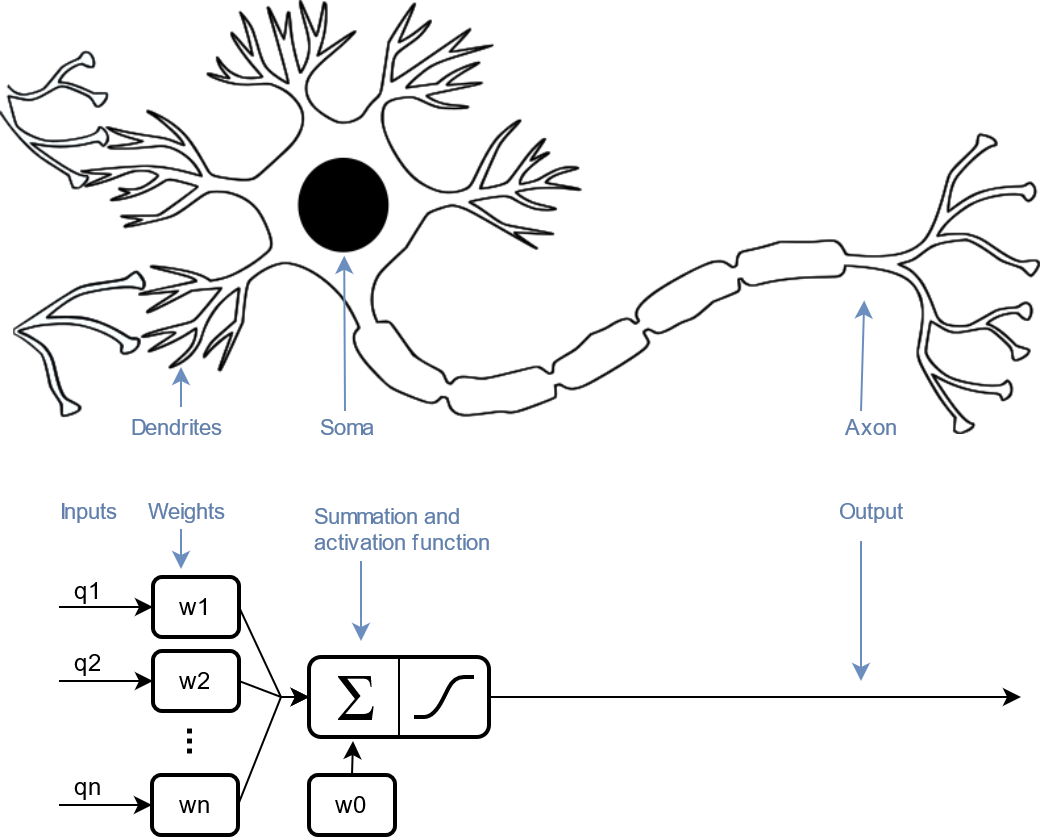
\includegraphics[width=\linewidth]{"../Chap2/Figures/Fig_neuron.png"}
	\caption{The artificial neuron has been modeled after the natural neuron. Inputs and weights act as the total nervous influx firing the dendrites. The collected values are summed, and a signal is activated if a threshold is overcome, as the soma does in a natural neuron. The output signal is conveyed through the axon.}
	\label{fig_neuron}
\end{figure}

\begin{algorithm}[!ht]
      \caption{Perceptron}\label{alg:perceptron}
      \begin{algorithmic}[1]
        \STATEx Let \( \overrightarrow{X^0} \) be the input vector of a first instance of variables \( (1, x_1^0, \cdots x_m^0) \), \( \overrightarrow{W^0} \) the corresponding weights randomly initialized \( (w_0^0, w_1^0, \cdots w_m^0) \) with \(w_0^0\) a bias, and $\sigma^{0, pred}$ the output predicted binary class. 
        \STATE The summation function is computed: 
        \begin{equation}
            \overrightarrow{W^0} \cdot \overrightarrow{X^0} = \sum_{k \in [0,m]} w_k^0 x_k^0
        \end{equation}
        \STATE This result is processed by an activation function which determines whether the neuron will be fired or not, i.e., whether one or the other class will be predicted. $\sigma^{0,pred}$ = 1 corresponds to one class, and $\sigma^{0,pred}$ = 0 to the other. 
        \begin{equation}
            \sigma^{0,pred} = 
            \begin{cases}
                1 & \text{if} \ \overrightarrow{W^0} \cdot \overrightarrow{X^0} > \theta,\\
                0 & \text{otherwise}
            \end{cases}
        \end{equation}
        \algstore{alg1}
      \end{algorithmic}
\end{algorithm}

\clearpage

\begin{algorithm}
      \begin{algorithmic}[1]
        \algrestore{alg1}
        \STATE This prediction $\sigma^{0,pred}$ is compared to the actual class $\sigma^{0,actual}$. 
        \STATEx If the class is correctly predicted, then weights are retained.
        \STATEx Else, they are updated: 
        \begin{equation}
            \overrightarrow{W^1} = \overrightarrow{W^0} + \eta \ \epsilon^0 \ \overrightarrow{X^0}
        \end{equation}
        \STATEx with $\eta$ the learning rate $\in$ [0,1], and $\epsilon$ the error function such as 
        \begin{equation}
            \epsilon^0 = \sigma^{0,actual} - \sigma^{0,pred}
        \end{equation}
      %   \STATEx \textit{In Adaline, weights are adjusted early and in a continuous way, before being processed by the activation function: \(\epsilon^0 = \frac{\partial \frac{1}{2}(\sigma^{0,actual} - \overrightarrow{W^0} \cdot \overrightarrow{X^0})^2}{\partial \overrightarrow{W^0}}= \sigma^{0,actual} - \overrightarrow{W^0} \cdot \overrightarrow{X^0}\)}.
        \STATE The algorithm is repeated with another example $\overrightarrow{X^1}$, and so on until it has gone through the whole batch of the training set. If weights still need to be updated, one can go over it again, for a determined number of epochs or until the average error is under a given value. Then the perceptron is considered trained, and ready to correctly predict a class $\sigma$ with the retained weights.
      \end{algorithmic}
\end{algorithm}

\begin{tcolorbox}[colback=white,colframe=black, colbacktitle=white, coltitle=black, breakable, title=\textbf{Example 1} Athlete classification with a perceptron, label=example1]
      \phantomsection\hypertarget{example1}
      N.B. The code for running this example is available on the thesis repository \url{https://github.com/davidpagnon/These_David_Pagnon/blob/main/Thesis/Chap2/perceptron.py}.
      \tcblower
      Let's consider force-velocity test results as an input
      \setlength{\belowdisplayskip}{0pt} \setlength{\belowdisplayshortskip}{0pt}
      \setlength{\abovedisplayskip}{0pt} \setlength{\abovedisplayshortskip}{0pt}
      \begin{flalign*}
      \overrightarrow{X} = (1, velocity \ (m/s), force \ (hN) ), && 
      \end{flalign*}
      and the classification of an athlete as "good" or "bad" as an output
      \(\sigma = 1 \ or \ 0. \)\newline
      A batch of training data, i.e., example data the perceptron will learn from, could be: 
      \[ \bigl\{(\overrightarrow{X^i}, \sigma^{i, actual})\bigr\}_{i\in [0,4]}
      = \bigl\{\bigl((1, 1, 5), 1\bigr),
      \bigl((1, 2, 3), 0\bigr),
      \bigl((1, 7, 1), 1\bigr),
      \bigl((1, 4, 1), 0\bigr),
      \bigl((1, 5, 4), 1\bigr)\bigr\}. \]
      
      Let's randomly initialize weights at \(\overrightarrow{W^0} =  (-9, 1, 3) \), take a threshold $\theta$=0.1, and a learning rate $\eta$ = 0.3.\newline
        
      \textbf{The first instance} of the training set gives: 
      \begin{flalign*}
      \overrightarrow{W^0} \cdot \overrightarrow{X^0} = \sum\nolimits_{k \in [0,2]} w_k^0 x^0_k = -9 \times 1+ 1 \times 1 + 3 \times 5 =7.&&
      \end{flalign*}
      Now \(\overrightarrow{W^0} \cdot \overrightarrow{X^0} = 7 > \theta = 0.1\), so $\sigma^{0, pred} = 1$.\newline
      \(\sigma^{0, actual} = 1 = \sigma^{0, pred} \), so the prediction is true and weights don't need to be updated. \newline
      As a consequence, \(\overrightarrow{W^1} = \overrightarrow{W^0} = (-9, 1, 3).\)\newline
      
      \textbf{The second instance} gives \(\overrightarrow{W^1} \cdot \overrightarrow{X^1} = (-9, 1, 3) \cdot (1,2,3) = 2 > \theta = 0.1\), so $\sigma^{1, pred} = 1$. \newline
      But \(\sigma^{1, actual} = 0 \neq \sigma^{1, pred} = 1\), so weights need to be updated.\newline
      The error is \(\epsilon^1 = \sigma^{1,actual} - \sigma^{1,pred} = 0-1 = -1\).\newline
      As a consequence, \(\overrightarrow{W^2} = \overrightarrow{W^1} + \eta \ \epsilon^1 \ \overrightarrow{X^1} = (-9, 1, 3)  + 0.1 \times (-1) \times (1,2,3) = (-9.3,0.4,2.1).\)\newline
      
      \textbf{Third instance}: \(\overrightarrow{W^2} \cdot \overrightarrow{X^2} = (-9.3,0.4,2.1) \cdot (1,7,1) = 3-4.4 < 0.1\), so $\sigma^{2, pred} = 0$. \newline
      \(\sigma^{2, actual} = 1 \neq \sigma^{2, pred} = 0\), so weights need to be updated.\newline 
      \(\epsilon^2 = \sigma^{2,actual} - \sigma^{2,pred} = 1\).\newline
      \(\overrightarrow{W^3} = \overrightarrow{W^2} + \eta \ \epsilon^2 \ \overrightarrow{X^2} = (-9.3,0.4,2.1) + 0.1 \times 1 \times (1,7,1) = (-9,2.5,2.4).\)\newline
      
      \textbf{Fourth instance}: \(\overrightarrow{W^3} \cdot \overrightarrow{X^3} = (-9,2.5,2.4) \cdot (1,4,1) = 3.4 > 0.1\), so $\sigma^{3, pred} = 1$. \newline
      \(\sigma^{3, actual} = 0 \neq \sigma^{3, pred} = 1\), so weights need to be updated.\newline
      \(\epsilon^3 = \sigma^{3,actual} - \sigma^{3,pred} = -1\).\newline
      \(\overrightarrow{W^4} = \overrightarrow{W^3} + \eta \ \epsilon^3 \ \overrightarrow{X^3} = (-9,2.5,2.4) + 0.1 \times (-1) \times (1,4,1) = (-9.3,1.3,2.1).\)\newline
      
      \newpage

      \textbf{Fifth instance}: \(\overrightarrow{W^4} \cdot \overrightarrow{X^4} = (-9.3,1.3,2.1) \cdot (1, 5, 4) = 17.6 > 8\), so $\sigma^{4, pred} = 1$. \newline
      \(\sigma^{4, actual} = 1 = \sigma^{4, pred} = 1\), so weights don't need to be updated.\newline
      \(\overrightarrow{W^5} = \overrightarrow{W^4} = (-9.3,1.3,2.1) (Figure~\ref{fig_perceptron}). \)\newline

      \textbf{Next instances}: Once we have gone over the batch of training data, if the average error is below a given value, we can assume that the perceptron is trained. If not, we can use the next batch to pursue training. If it still didn't converge after all batches, we can iterate over all training data again, for a given number of times. If results are still not satisfying, either the data are not linearly separable, or the training sample is not large enough or of good enough quality. In our case, it seems like our example data have allowed us to correctly separate good and bad athletes based on their force and velocity test results (Figure~\ref{fig_perceptron}).

      {
      \begin{center}
      \def\svgwidth{1\columnwidth}
      \fontsize{10pt}{10pt}\selectfont
      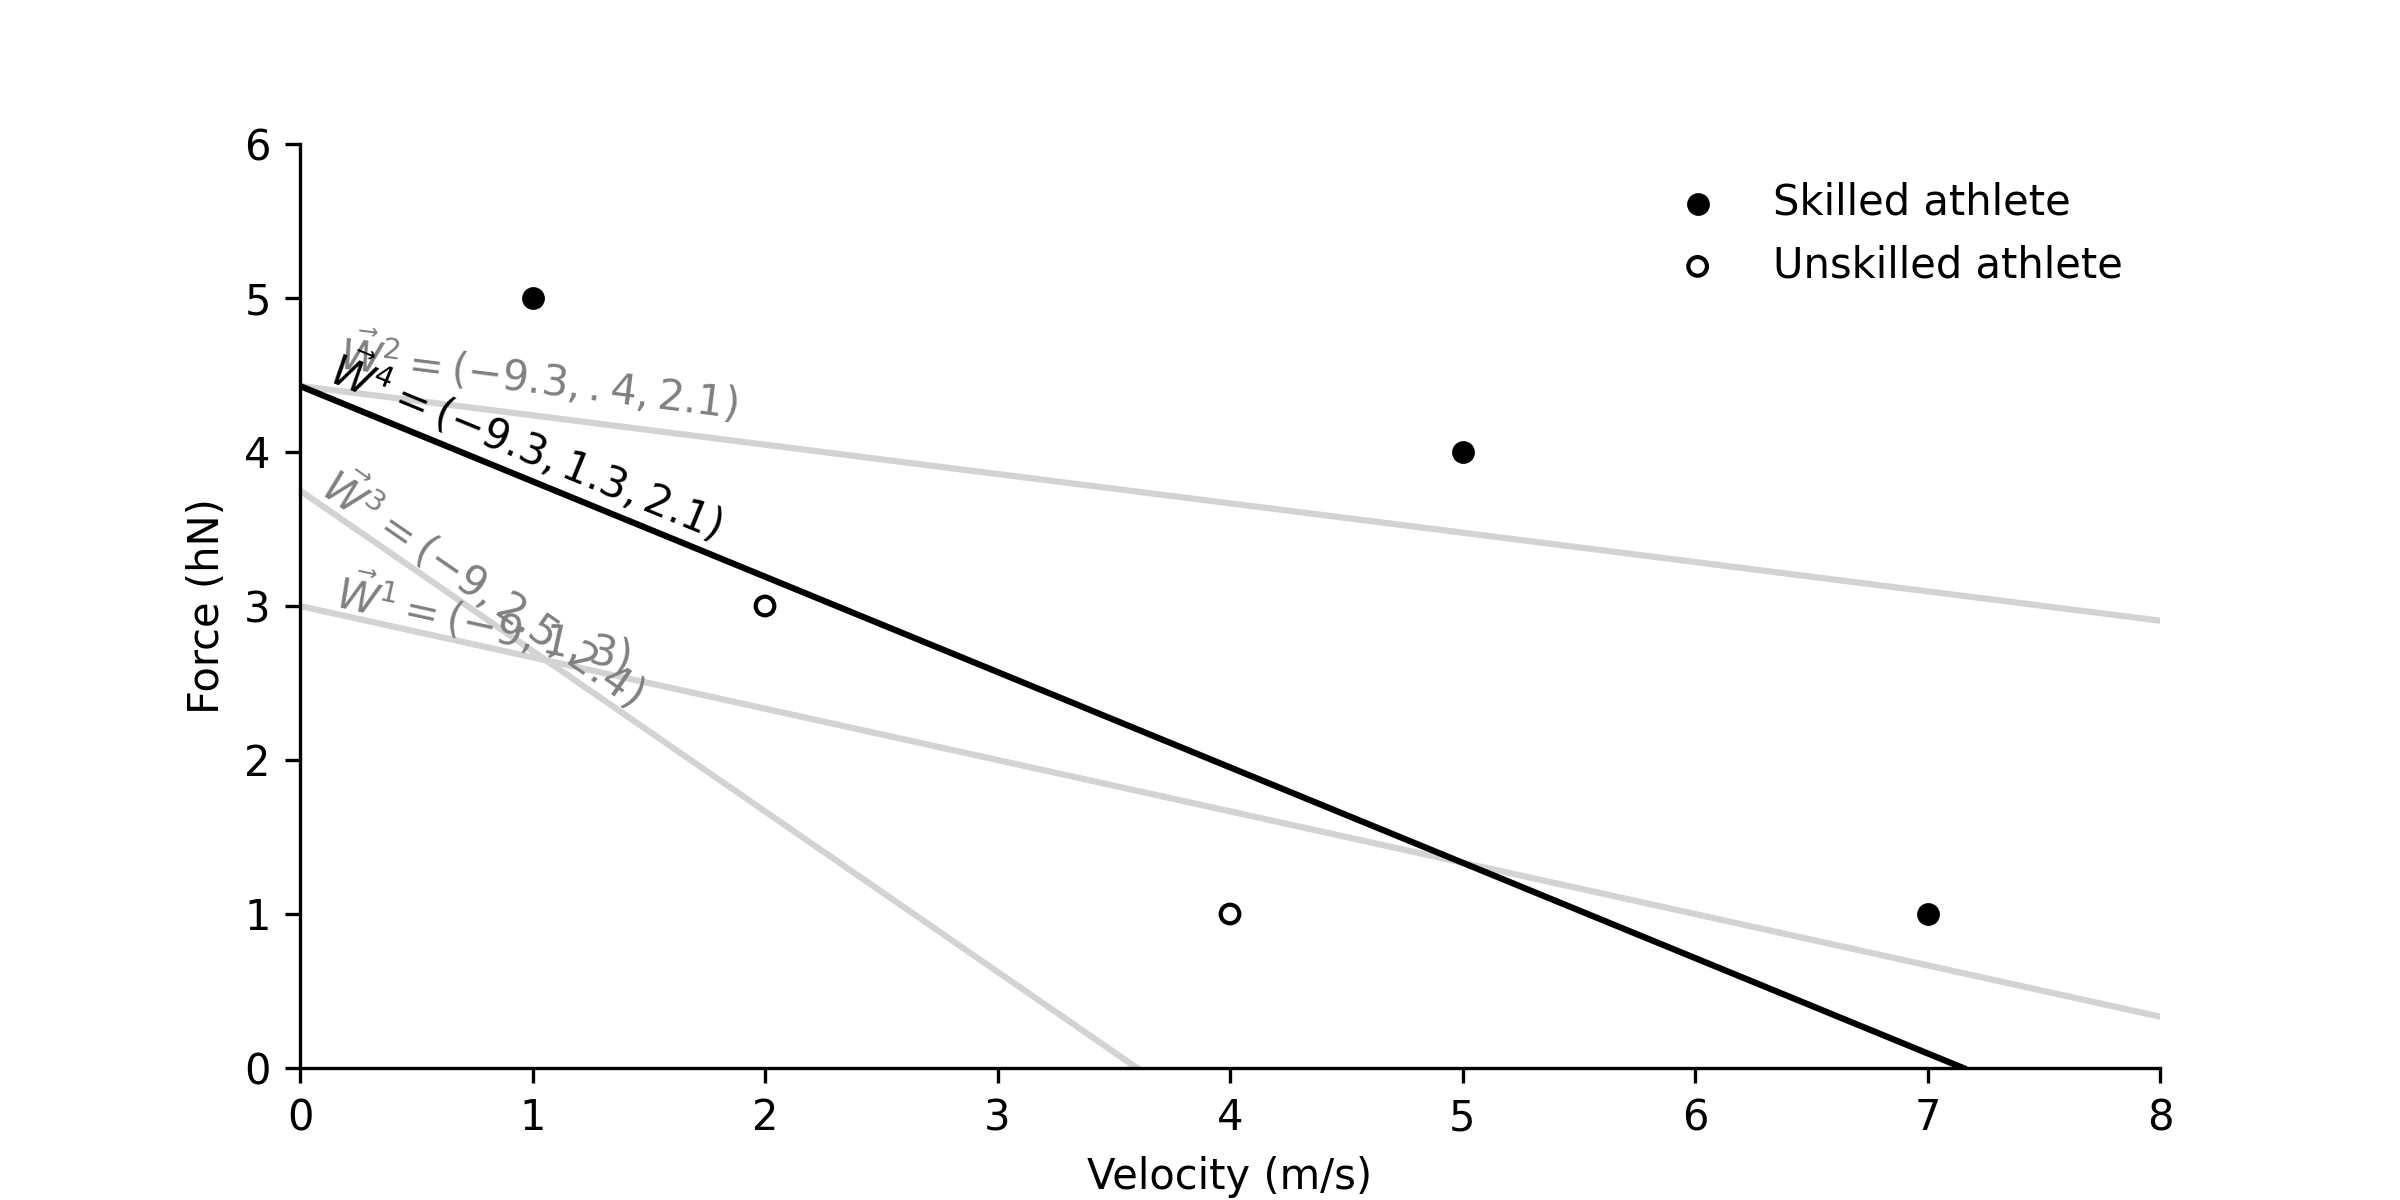
\includegraphics[width=\linewidth]{"../Chap2/Figures/Fig_perceptron.png"}
      \end{center}
      \captionof{figure}{Classification of athletes as "good" (black dot) or "bad" (circle) according to their Force-Velocity results. Weights are adjusted (grey lines), until the perceptron classifies athletes correctly (black line.)}
      \label{fig_perceptron}
      }
\end{tcolorbox}

Nevertheless, it often takes a lot of iterations over good quality training data for the perceptron to converge. Moreover, it does converge if and only if the data are linearly separable, i.e., if they can be separated with a straight line \cite{Novikoff1963} (see Figure~\ref{fig_linearly_sep}). Some fundamental problems such as the exclusive OR (XOR) gate can't be solved with a basic single layer ANN \cite{Minsky1969}. This constituted one of the early setbacks for AI. Then, the high computational cost of these approaches, combined with the complexity of common-sense problems, hampered the trust in learning methods. Vision and language problems require enormous amounts of information, and can't be solved with a simple dictionary (for example, "the spirit is willing but the flesh is weak" becomes "the vodka is good but the meat is rotten" when translated back and forth from English to Russian.) Overinflated promises and expectations, followed by disappointment in academia and industries, lead to cuts in fundings, and eventually loss of skills in the 1970s: this is refered to as the first AI winter.

% Adaline (gradient descent)
% Logistic regression (softmax)
% Multi-layer, backpropagation
% second winter, from late 1980s to early 1990s. Same reasons as the first one, i.e., unrealisitic expectations confronted with unexpected technical difficulties.
% vanishing gradient, overfitting (data augmentation, dropout, batch normalization), 
% CNN
% Deep learning
% Classification, detection, segmentation
% transfer learning

% train / test, accuracy loss
% layers, batch size, epochs, activation



% This is the idea behind the multilayer perceptron (MLP), which was invented in 1969 \cite{Rumelhart1986}. This is a neural network composed of several layers of neurons (perceptron = learning unit), which can be used to classify data in a more complex way. For example, if one wants to classify athletes according to their performance in a 100m sprint, they could use the time, the force-velocity results, the body mass, the height, the age, etc. as input variables. The first layer of neurons would be used to classify the athletes according to their force-velocity results, the second layer would classify them according to their time, and so on. The output layer would then be used to classify them according to their performance.

\begin{figure}[hbtp]
	\centering
	\def\svgwidth{1\columnwidth}
	\fontsize{10pt}{10pt}\selectfont
	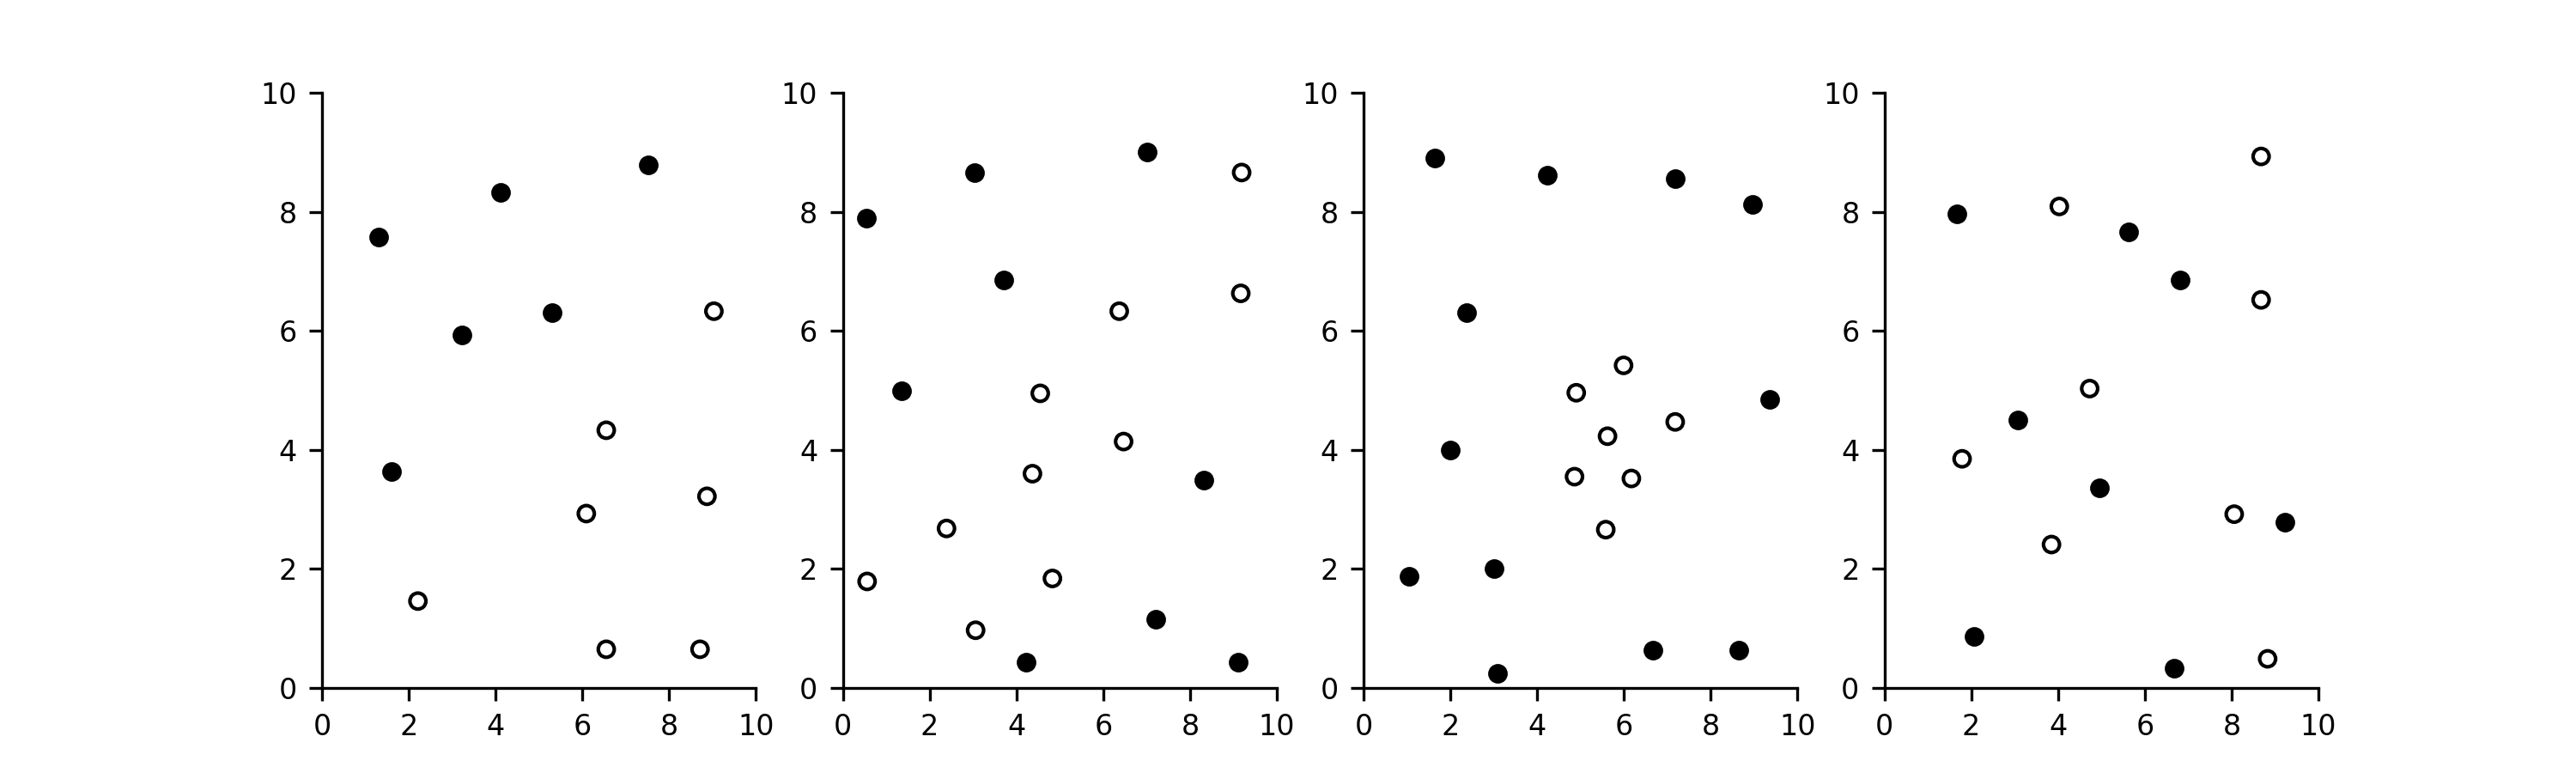
\includegraphics[width=\linewidth]{"../Chap2/Figures/Fig_linearly_sep.png"}
	\caption{Single layer artificial neural networks such as the perceptron can only classify linearly separable data. (a) is linearly separable. (b) is not linearly separable. However, data are contained in an ellipse. The equation of an ellipse is of the form \(a \times x^2+b\times y^2=1\), so if we transform the feature variables into \(X=x^2\) and \(Y=y^2\), the data become linearly separable. (c) is equivalent to a fundamental XOR gate, and is not linearly separable, which was part of the reasons for the first AI winter. It can either be solved by combining several layers of artificial neurons, or by complex kernel tricks which map the data from the original space into a higher dimensional space where they become linearly separable. (d) is not linearly separable. AI: Artificial Intelligence. XOR: Exclusive OR.} 
	\label{fig_linearly_sep}
\end{figure}

%Adaline \cite{Widrow1960} is an improved version of the perceptron, which introduces the concept of gradient descent. It converges faster as weights are adjusted early and in a continuous way, by directly using the result of the summation function instead of processing it with a binary activation function (see Algorithm~\ref{alg:perceptron}). As a consequence, the weights are more or less heavily adjusted depending on how large the error is, in an adaptive way (hence its name, which stands for Adaptive Linear Element.) 
% The logistic regression \cite{} uses a softmax activation function, which allows for a a classification over more than two classes. These three algorithms form the most basic supervised learning algorithms (i.e., trained based on labels representing the expected output rather than fully automatically, without  supervision,) and are refered to as single layer Artificial Neural Network (ANN.) 

% Non-linear problems can either be solved by using multi-layer neural networks with backpropagation, or by using kernel tricks \cite{Aizerman1964}. Kernel tricks consist in mapping the input data into a higher dimensional space, where they become linearly separable. However, although the concepts had been introduced early, they have not been connected to this particular problem until much later.




% learning rate, the number of iterations, the number of layers, the number of neurons per layer, the activation function, the regularization, etc. to get a better result. 

% Learning rate, threshold
% training data size (and quality), number of epochs to run on a batch (i.e., a subset of the training data)
% activation function, error (gradient descent)
% only linearly separable
% multilayer


















  



% \begin{figure}[hbtp]
% 	\centering
% 	\def\svgwidth{1\columnwidth}
% 	\fontsize{10pt}{10pt}\selectfont
% 	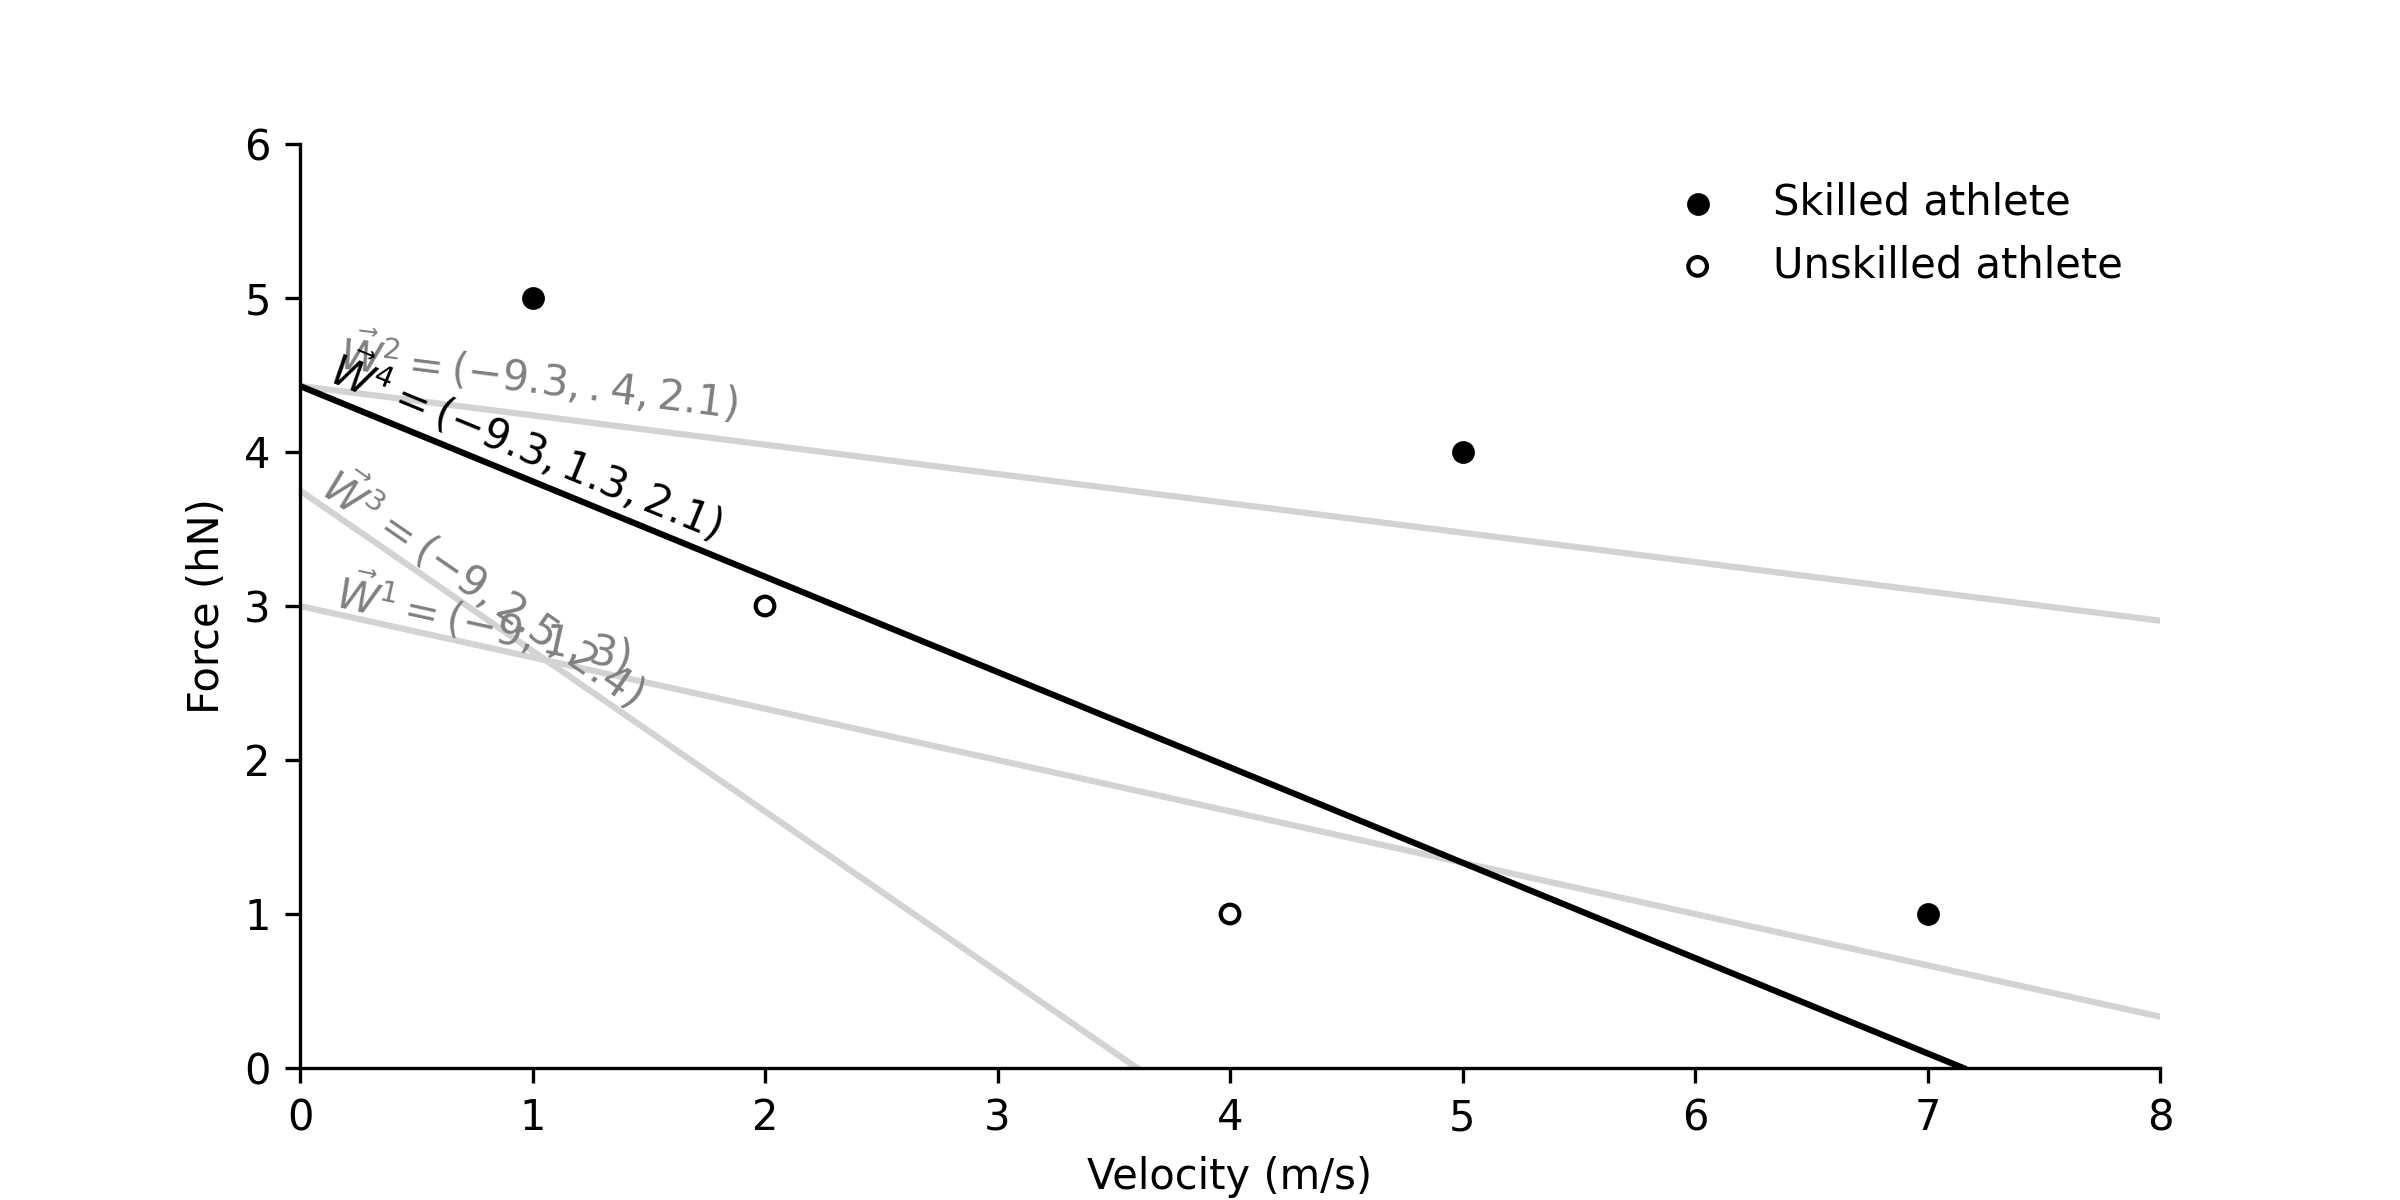
\includegraphics[width=\linewidth]{"../Chap2/Figures/Fig_perceptron.png"}
% 	\caption{Classification of athletes as "good" (black dot) or "bad" (circle) according to their Force-Velocity results. Weights are adjusted (grey lines), until the perceptron classifies athletes correctly (black line.)}
% 	\label{fig_perceptron}
% \end{figure}

% % En tikz
% \begin{figure}
% \centering
% \begin{tikzpicture}[x=0.5cm, y=0.5cm]
%     \draw[thick,->] (0,0) -- (0,6) node[anchor=south east] {Force (hN)};
%     \draw[thick,->] (0,0) -- (10,0) node[anchor=north west] {velocity (m/s)};
%     \foreach \x in {0,1,2,3,4,5,6,7,8,9}
%         \draw (\x,1pt) -- (\x,-1pt) node[anchor=north] {$\x$};
%     \foreach \y in {0,1,2,3,4,5}
%         \draw (1pt,\y) -- (-1pt,\y) node[anchor=east] {$\y$};
%     \foreach \Point in {(1,5), (5,4), (7,1)}{
%       \node at \Point {\textbullet};}
%     \foreach \Point in {(2,3), (4,1)}{
%       \node at \Point {$\circ$};}
%     % \node [green] at (5,4) {\textbullet};
%     % \node [red] at (2,3) {$\circ$};
%     \end{tikzpicture}
% \caption{Force-velocity results and classification.}
% \end{figure}

% % En matplotlib
% # Found ion https://stackoverflow.com/questions/19907140/keeps-text-rotated-in-data-coordinate-system-after-resizing
% import matplotlib.pyplot as plt
% import numpy as np
% plt.rcParams.update({'font.size': 8})
% #import matplotlib.mathtext as mathtext
% import matplotlib.text as mtext
% import matplotlib.transforms as mtransforms

% class RotationAwareAnnotation(mtext.Annotation):
%     def __init__(self, s, xy, p, pa=None, ax=None, **kwargs):
%         self.ax = ax or plt.gca()
%         self.p = p
%         self.pa = pa
%         if not pa:
%             self.pa = xy
%         self.calc_angle_data()
%         kwargs.update(rotation_mode=kwargs.get("rotation_mode", "anchor"))
%         mtext.Annotation.__init__(self, s, xy, **kwargs)
%         self.set_transform(mtransforms.IdentityTransform())
%         if 'clip_on' in kwargs:
%             self.set_clip_path(self.ax.patch)
%         self.ax._add_text(self)

%     def calc_angle_data(self):
%         ang = np.arctan2(self.p[1]-self.pa[1], self.p[0]-self.pa[0])
%         self.angle_data = np.rad2deg(ang)

%     def _get_rotation(self):
%         return self.ax.transData.transform_angles(np.array((self.angle_data,)), 
%                             np.array([self.pa[0], self.pa[1]]).reshape((1, 2)))[0]

%     def _set_rotation(self, rotation):
%         pass

%     _rotation = property(_get_rotation, _set_rotation)

% plt.figure(figsize=(8, 4))
% plt.axis([0, 8, 0, 6])
% plt.gca().spines['top'].set_visible(False)
% plt.gca().spines['right'].set_visible(False)
% plt.gca().set_xlabel('Velocity (m/s)')
% plt.gca().set_ylabel('Force (hN)')

% velocity_good = [1,5,7]
% force_good = [5,4,1]
% velocity_bad = [2,4]
% force_bad = [3,1]
% plt.scatter(velocity_good, force_good, s=20, edgecolors='k', facecolors='k', label = "Good athlete")
% plt.scatter(velocity_bad, force_bad, s=20, edgecolors='k', facecolors='none', label="Bad athlete")
% plt.legend(frameon=False)

% # First lines with first weights, with dash greyed lines and label
% W=[-9,  1,  3]
% x1 = np.array( [0, -W[0]/W[1]] )
% x2 = np.array( [-W[0]/W[2], 0] )
% plt.plot(x1,x2, 'lightgrey')
% RotationAwareAnnotation(r'$\vec{W}^1=(-9,1,3)$', 
%       xy=(.15,3.3), p=[-W[0]/W[1],0], pa=[0,-W[0]/W[2]], ax=plt.gca(), xytext=(2,-1), textcoords="offset points", va="top", c='grey', bbox=dict(facecolor='None', edgecolor='None'))
    
% W=[-9.3, .4,  2.1]
% x1 = np.array( [0, -W[0]/W[1]] )
% x2 = np.array( [-W[0]/W[2], 0] )
% plt.plot(x1,x2, 'lightgrey')
% RotationAwareAnnotation(r'$\vec{W}^2=(-9.3, .4,  2.1)$', 
%       xy=(.15,4.85), p=[-W[0]/W[1],0], pa=[0,-W[0]/W[2]], ax=plt.gca(), xytext=(2,-1), textcoords="offset points", va="top", c='grey', bbox=dict(facecolor='None', edgecolor='None'))

% W=[-9,  2.5, 2.4]
% x1 = np.array( [0, -W[0]/W[1]] )
% x2 = np.array( [-W[0]/W[2], 0] )
% plt.plot(x1,x2, 'lightgrey')
% RotationAwareAnnotation(r'$\vec{W}^3=(-9,2.5,2.4)$', 
%     xy=(.15,4), p=[-W[0]/W[1],0], pa=[0,-W[0]/W[2]], ax=plt.gca(), xytext=(2,-1), textcoords="offset points", va="top", c='grey', bbox=dict(facecolor='None', edgecolor='None'))

% W=[-9.3,  1.3, 2.1]
% x1 = np.array( [0, -W[0]/W[1]] )
% x2 = np.array( [-W[0]/W[2], 0] )
% plt.plot(x1,x2, 'k')
% RotationAwareAnnotation(r'$\vec{W}^4=(-9.3,  1.3, 2.1)$', 
%       xy=(.15,4.75), p=[-W[0]/W[1],0], pa=[0,-W[0]/W[2]], ax=plt.gca(), xytext=(2,-1), textcoords="offset points", va="top", bbox=dict(facecolor='None', edgecolor='None'))

% plt.savefig(r'D:\softs\github_david\These_David_Pagnon\Thesis\Chap2\Figures\Fig_perceptron', dpi=300)
% plt.show()















% \subsection{Application to object detection and localization}


\subsection{Pose detection}

Different architectures, different models, different datasets
Discriminative vs generative

\section{3D reconstruction}\label{sec:3D reconstruction}

While some approaches only rely on 2D pose estimation to infer 3D pose with another machine learning model, they are generally not considered to be sufficiently reliable. It is, then, important to use the input from several cameras, and to fuse their informations to obtain 3D coordinates.


\subsection{Pinhole camera model}

Voilà


\subsection{Calibration}

test


\subsection{Triangulation}

suite


\section{3D joint kinematics}

\subsection{Physically consistent model}

autre


\subsection{Scaling}

bref


\subsection{Inverse kinematics}

As opposed to forward kinematics \newline
Compare with 2D angles between 3 points \newline
Different methods (model based vs autres) for angles (cf mail starred)\newline




% import matplotlib.pyplot as plt
% import numpy as np
% plt.rcParams.update({'font.size': 8})

% # Place dots on graph on click and record position
% # adapted from https://stackoverflow.com/a/41825214/12196632
% fig = plt.figure()
% ax = fig.add_subplot(111)
% ax.set_xlim([0, 10])
% ax.set_ylim([0, 10])

% def onclick(event):
%     print(f'{event.xdata}, {event.ydata}')
%     plt.plot(event.xdata, event.ydata, 'o')
%     fig.canvas.draw()
% cid = fig.canvas.mpl_connect('button_press_event', onclick)
% plt.show()


% # Plot examples of linearly and non-liearly separable data
% fig, axs = plt.subplots(1,4,figsize=(10,3))
% plt.rcParams.update({'font.size': 8})

% axs[0].scatter([1.31,4.11,3.22,1.61,5.30,7.52], [7.58,8.33,5.93,3.63,6.31,8.79],s=20, edgecolors='k', facecolors='k')
% axs[0].scatter([6.55,8.71,8.87,9.03,6.55,2.21,6.09], [0.65,0.65,3.22,6.33,4.33,1.46,2.93],s=20, edgecolors='k', facecolors='None')
% axs[0].plot([0,10],[1,10])
% axs[0].text(0.5,0.5,'(a)')

% axs[1].scatter([1.65,4.23,2.38,1.05,3.08,8.65,9.35,8.97,6.67, 7.19,3.00,2.00], [8.91,8.61,6.31,1.87, 0.25,0.63,4.85,8.12,0.63,8.55,2.00,4.00],s=20, edgecolors='k', facecolors='k')
% axs[1].scatter([4.90,4.86,6.17,5.62,5.99,5.58,7.18], [4.96,3.55,3.52,4.23,5.42,2.66,4.47],s=20, edgecolors='k', facecolors='None')
% t = np.linspace(0, 2*np.pi, 100)
% axs[1].plot(6+1.8*np.cos(t) , 4+2*np.sin(t),'-')
% axs[1].text(0.5,0.5,'(b)')

% axs[2].scatter([0.54,3.04,7.01,3.70,1.35,4.23,7.21,9.11,8.32], [7.90, 8.66,9.01,6.85,5.00,0.44,1.16,0.43,3.49],s=20, edgecolors='k', facecolors='k')
% axs[2].scatter([0.56,2.39,4.55,9.19,6.37,6.47,3.06,4.37,9.17,4.83], [1.79,2.68,4.95,8.66,6.33,4.14,0.97,3.60,6.63,1.84],s=20, edgecolors='k', facecolors='None')
% axs[2].plot([0,10],[2,10])
% axs[2].plot([3,10],[0,5], c='tab:blue')
% axs[2].text(0.5,0.5,'(c)')

% axs[3].scatter([1.67,3.08,6.81,9.23,6.67,2.06,4.96,5.62], [7.96,4.50,6.85,2.79,0.33,0.87,3.36,7.66],s=20, edgecolors='k', facecolors='k')
% axs[3].scatter([8.68,1.79,3.85,4.73,4.03,8.06,8.83,8.68], [6.52,3.85,2.41,5.03,8.09,2.92,0.49,8.93],s=20, edgecolors='k', facecolors='None')
% axs[3].text(5,3.5,'?',fontsize=70, **{'color':'tab:blue', 'fontfamily':'monospace'})
% axs[3].text(0.5,0.5,'(d)')

% for ax in axs:
%     ax.set_xlim([0, 10])
%     ax.set_ylim([0, 10])
%     ax.spines['top'].set_visible(False)
%     ax.spines['right'].set_visible(False)

% fig.savefig(r'D:\softs\github_david\These_David_Pagnon\Thesis\Chap2\Figures\Fig_linearly_sep', dpi=300)
% fig.show()
